\documentclass[main.tex]{subfiles}
\begin{document}

\section{Voorbeelden in metrische ruimten}
\label{sec:voorb-metr-ruimt}


\subsection{De discrete metriek}
\label{sec:de-discrete-metriek}

\begin{vb}
  Zij $X$ een willekeurige, niet-lege verzameling.
  De \term{discrete metriek} of \term{triviale metriek} op $X$ wordt gegeven als volgt.
  \[
  d_{X}:\ X \times X \rightarrow \mathbb{R}^{+}:\ (x,y) \mapsto
  \begin{cases}
    0 &\text{ als } x = y\\
    1 &\text{ als } x \neq y
  \end{cases}
  \]
  $X,d_{X}$ vormt een metrische ruimte.
\end{vb}

\begin{st}
  Elke verzameling is begrensd voor de discrete metriek.

  \begin{proof}
    Inderdaad, de afstand tussen twee elementen is nooit groter dan $1$.
  \end{proof}
\end{st}

\begin{vb}
  Een open bol rond $x\in \mathbb{R}$ met straal $\delta\in \mathbb{R}_{0}^{+}$ voor de gewone metriek ziet eruit als volgt:
  \[ B(x,\delta) = 
  \begin{cases}
    \{x\} &\text{ als } r\le 1\\
    X &\text{ als } r > 1
  \end{cases}
  \]
\extra{bewijs}
\end{vb}

\begin{st}
  Elke deelverzameling $A$ van een verzameling $X$ is zowel open als gesloten voor de triviale metriek.
\extra{bewijs}
\end{st}


\begin{vb}
  Voor de triviale metriek $d_{X}$ voor een verzameling $X$, is elke functie $f:\ X \rightarrow Y$ met $Y,d_{Y}$ een metrische ruimte, continu.
\extra{bewijs}
\end{vb}

\subsection{Metrieken op $\mathbb{R}$}
\label{sec:metrieken-op-mathbbr}

\subsubsection{De gewone metriek op $\mathbb{R}$}
\label{sec:de-gewone-metriek}

\begin{vb}
  $\mathbb{R}$, uitgerust met een metriek gebaseerd op de absolute-waardefunctie, is een metrische ruimte:
  \[ d:\ \mathbb{R}\times\mathbb{R}\rightarrow (x,y) \mapsto d(x,y)=|x-y| \]
  Men noemt dit de \term{gewone metriek op $\mathbb{R}$}.
\extra{bewijs}
\end{vb}

\begin{opm}
  $\mathbb{R}$ is niet begrensd voor $d$.
\extra{bewijs}
\end{opm}

\begin{vb}
  Een open bol rond $x\in \mathbb{R}$ met straal $\delta\in \mathbb{R}_{0}^{+}$ voor de gewone metriek ziet eruit als volgt:
  \[ B(x,\delta) = \interval[open]{x-\delta}{x+\delta} \]
  \begin{figure}[H]
    \centering
    \begin{tikzpicture}[scale=1.5]
      \draw[latex-latex] (-1.5,0) -- (1.5,0);
      \draw[color=black] (0pt,3pt) -- (0pt,-3pt) node[below] {$a$};
      \draw[(-),thick,color=red] (-1,0) -- (1,0);
    \end{tikzpicture}
    \caption{Een open bol in $\mathbb{R},d$}
  \end{figure}
\extra{bewijs}
\end{vb}


\subsubsection{De $d_1$-metriek op $\mathbb{R}$}
\label{sec:d_1-metriek-op}

\begin{vb}
  $\mathbb{R}$, uitgerust met de volgende functie als metriek, is een metrische ruimte:
  \[ d_{1}:\ \mathbb{R}\times\mathbb{R}\rightarrow (x,y) \mapsto d_{1}(x,y)=\frac{|x-y|}{1+|x-y|} \]
  \begin{proof}
    We gaan elke eigenschap van een metrische ruimte na.
    \begin{itemize}
    \item $d$ is symmestrisch.
      Dit volgt meteen uit de symmetrie van de gewone metriek op $\mathbb{R}$.
    \item $d$ is nu als en slechts als de argumentien nul zijn.
      Dit volgt uit dezelfde eigenschap van de gewone metriek op $\mathbb{R}$
    \item $d$ voldoet aan de driehoeksongelijkheid:\\
      Kies $x,y,z \in \mathbb{R}$ en houdt de driehoeksongelijkheid voor de gewone metriek op $\mathbb{R}$ in het achterhoofd.
      Merk op dat de functie $f$ als volgt stijgend is.
      \[ f:\ \mathbb{R}^{+} \rightarrow \mathbb{R}^{+}:\ t \mapsto \frac{t}{1+t} \]
      \begin{align*}
        d_{1}(x,y)
        &= f(|x-y|)\\
        &\le f(|x-z|+|z-y|)\\
        &= \frac{|x-z|+|z-y|}{1+|x-z|+|z-y|}\\
        &= \frac{|x-z|}{1+|x-z|+|z-y|}+\frac{|z-y|}{1+|x-z|+|z-y|}\\
        &\le \frac{|x-z|}{1+|x-z|}+\frac{|z-y|}{1+|z-y|}\\
        &= d_{1}(x,z) + d_{1}(z,y)
      \end{align*}
    \end{itemize}
  \end{proof}
\end{vb}

\begin{st}
  Voor de $d_{1}$ metriek is $\mathbb{R}$ begrensd.
  \begin{proof}
    Kies willekeurig $x,y\in\mathbb{R}$ en kies $M=1\in \mathbb{R}^{+}$, dan geldt het volgende:
    \[ d_{1}(x,y) = \frac{|x-y|}{1+|x-y|} < M \]
  \end{proof}
\end{st}
\extra{vindt de diameter}

\begin{vb}
  Een open bol rond $x\in \mathbb{R}$ met straal $\delta\in \mathbb{R}_{0}^{+}$ voor de $d_{1}$-metriek ziet eruit als volgt:
  \[ B(x,\delta) = 
  \begin{cases}
    \mathbb{R} &\text{ als } r \ge 1\\
    \interval[open]{x-\frac{r}{1-r}}{x+\frac{r}{1-r}}
  \end{cases}
  \]
\extra{bewijs}
\end{vb}

\begin{st}
  Een deelverzameling $A$ van $\mathbb{R}$ is $d_{1}$-open als en slechts als ze open is voor de gewone metriek.
\extra{bewijs}
\end{st}

\subsubsection{De $d_2$-metriek op $\mathbb{R}$}
\label{sec:d_2-metriek-op}

\begin{vb}
  $\mathbb{R}$, uitgerust met de volgende functie als metriek, is een metrische ruimte:
  \[ d_{2}:\ \mathbb{R}\times\mathbb{R}\rightarrow (x,y) \mapsto d_{2}(x,y)=\left| \frac{x}{1+|x|} - \frac{y}{1+|y|} \right| \]
\extra{bewijs}
\end{vb}

\begin{st}
  Voor de $d_{2}$ metriek hierboven is $\mathbb{R}$ begrensd.
\extra{bewijs}
\end{st}
\extra{vindt de diameter}

\mst{Een deelverzameling $A$ van $\mathbb{R}$ is $d_{2}$-open als en slechts als ze open is voor de gewone metriek.}

\begin{vb}
  $\mathbb{R},d_{2}$ en $\interval[open]{-1}{1},d$ zijn isometrisch.
\extra{bewijs} 
\end{vb}

\subsubsection{De $d_3$-metriek op $\mathbb{R}$}
\label{sec:d_3-metriek-op}

\begin{vb}
  De functie $d_{3}$ als volgt is een metriek voor $\mathbb{R}$.
  \[
  d_{3}:\ \mathbb{R} \times \mathbb{R} \rightarrow \mathbb{R}^{+}:\ (x,y) \mapsto
  \begin{cases}
    d_{3}(x,y) = |x-y| &\text{ als } x\neq 0 \neq y\\
    d_{3}(x,0) = d(0,x) = 1 + |x| &\text{ als } x \neq 0\\
    d_{3}(0,0) = 0
  \end{cases}
  \]
\extra{bewijs}
\end{vb}


\subsection{Metrieken op $\mathbb{R}^p$}
\label{sec:metr-op-mathbbrp}

\subsubsection{De gewone metriek op $\mathbb{R}^p$}
\label{sec:gewone-metriek-op}

\begin{vb}
  $\mathbb{R}^{p}$, uitgerust met de volgende functie als metriek, is een metrische ruimte:
  \[ d:\ \mathbb{R}^{p}\times\mathbb{R}^{p}\rightarrow (x,y) \mapsto d(x,y)=\|x-y\| \]
  We noemen dit de \term{gewone metriek} of \term{euclidische metriek} op $\mathbb{R}^{p}$.
  \extra{bewijs}
  \begin{figure}[H]
    \centering
    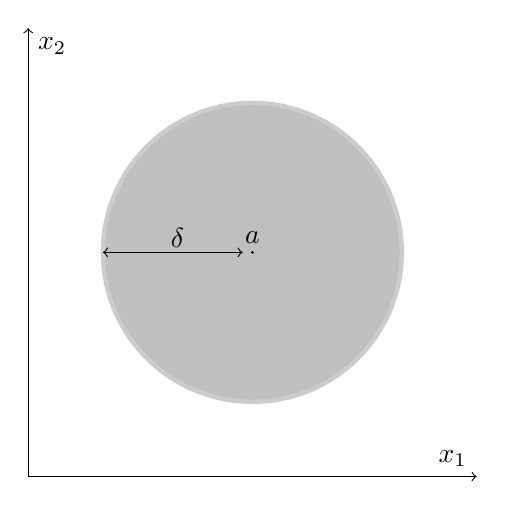
\begin{tikzpicture}
      \begin{axis}[ 
        ticks=none,
        axis lines = middle,
        axis line style={->},
        ymin=0, ymax=3,
        xmin=0, xmax=3,
        xlabel={$x_{1}$},
        ylabel={$x_{2}$},
        axis equal image,
        disabledatascaling
        ]
        \filldraw [ultra thick,fill=black!25!white, draw=black!20!white] (1.5,1.5) circle [radius=1];
        \fill [fill=black] (1.5,1.5) circle [radius=0.01];
        \draw (1.5,1.6) node {$a$};
        \draw (1.5,1.5) node {} edge[<->] (0.5,1.5);
        \draw (1,1.6) node {$\delta$};
      \end{axis}
    \end{tikzpicture}
    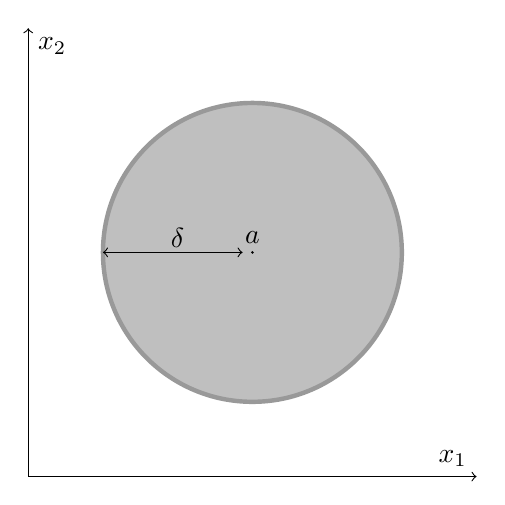
\begin{tikzpicture}
      \begin{axis}[ 
        ticks=none,
        axis lines = middle,
        axis line style={->},
        ymin=0, ymax=3,
        xmin=0, xmax=3,
        xlabel={$x_{1}$},
        ylabel={$x_{2}$},
        axis equal image,
        disabledatascaling
        ]
        \filldraw [ultra thick,fill=black!25!white, draw=black!40!white] (1.5,1.5) circle [radius=1];
        \fill [fill=black] (1.5,1.5) circle [radius=0.01];
        \draw (1.5,1.6) node {$a$};
        \draw (1.5,1.5) node {} edge[<->] (0.5,1.5);
        \draw (1,1.6) node {$\delta$};
      \end{axis}
    \end{tikzpicture}
    \caption{Een open bol en een gesloten bol in $\mathbb{R}^{2},d$}
  \end{figure}
\end{vb}

\subsubsection{De $d_1$- of city block metriek op $\mathbb{R}^p$}
\label{sec:de-d_1-city}

\begin{vb}
  $\mathbb{R}^{p}$, uitgerust met de volgende functie als metriek, is een metrische ruimte:
  \[ d_{1}:\ \mathbb{R}^{p}\times\mathbb{R}^{p}\rightarrow (x,y) \mapsto d_{1}(x,y)=\sum_{i=1}^{p}|x_{i}-y_{i}| \]
  We noemen dit de \term{city block metriek} of \term{taxicab metriek}.
\extra{bewijs}
  \begin{figure}[H]
    \centering
    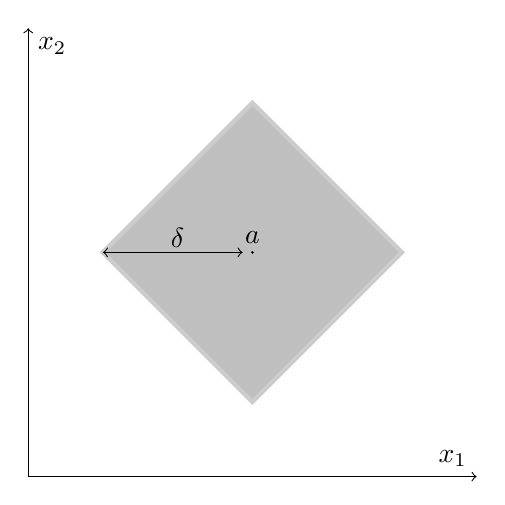
\begin{tikzpicture}
      \begin{axis}[ 
        ticks=none,
        axis lines = middle,
        axis line style={->},
        ymin=0, ymax=3,
        xmin=0, xmax=3,
        xlabel={$x_{1}$},
        ylabel={$x_{2}$},
        axis equal image,
        disabledatascaling
        ]
        \filldraw[ultra thick,fill=black!25!white, draw=black!20!white] (0.5,1.5) -- (1.5,2.5) -- (2.5,1.5) -- (1.5,0.5) -- cycle;
        \fill [fill=black] (1.5,1.5) circle [radius=0.01];
        \draw (1.5,1.6) node {$a$};
        \draw (1.5,1.5) node {} edge[<->] (0.5,1.5);
        \draw (1,1.6) node {$\delta$};
      \end{axis}
    \end{tikzpicture}
    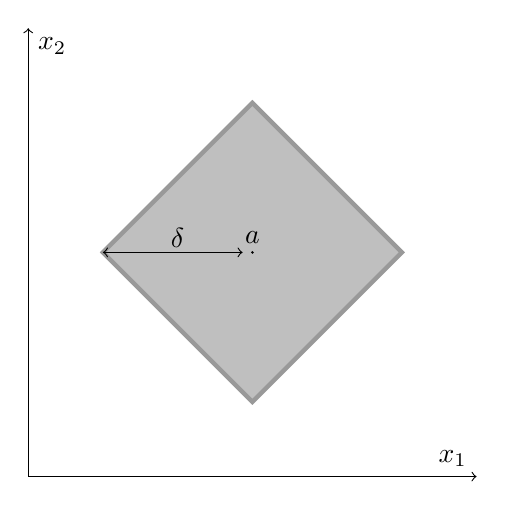
\begin{tikzpicture}
      \begin{axis}[ 
        ticks=none,
        axis lines = middle,
        axis line style={->},
        ymin=0, ymax=3,
        xmin=0, xmax=3,
        xlabel={$x_{1}$},
        ylabel={$x_{2}$},
        axis equal image,
        disabledatascaling
        ]
        \filldraw[ultra thick,fill=black!25!white, draw=black!40!white] (0.5,1.5) -- (1.5,2.5) -- (2.5,1.5) -- (1.5,0.5) -- cycle;
        \fill [fill=black] (1.5,1.5) circle [radius=0.01];
        \draw (1.5,1.6) node {$a$};
        \draw (1.5,1.5) node {} edge[<->] (0.5,1.5);
        \draw (1,1.6) node {$\delta$};
      \end{axis}
    \end{tikzpicture}
    \caption{Een open bol en een gesloten bol in $\mathbb{R}^{2},d_{1}$}
  \end{figure}
\end{vb}

\begin{st}
  Elke deelverzameling $A\subseteq \mathbb{R}^{p}$ is open voor de gewone metriek als en slechts als ze $d_{1}$-open is.

  \begin{proof}
    We moeten bewijzen dat er voor elke open bol $B(x,r)$ voor de gewone metriek een $d_{1}$-open bol $B_{1}(x,r_{1})$ bestaat met hetzelfde middelpunt die erin ligt en omgekeerd.
    \begin{itemize}
    \item $\Rightarrow$\\
      Kies een open bol $B(x,r)$ voor de gewone metriek.
      $B_{1}(x,r)$ voor de $d_{1}$ metriek is er dan een deel van:
      \[ \forall x,y\in A:\ d_{1}(x,y)^{2} = \left(\sum_{i=1}^{p}|x_{i}-y_{i}|\right)^{2} \ge \sum_{i=1}^{p}|x_{i}-y_{i}| = d(x,y)^{2} \]
      Als $d_{1}(x,y)$ dus kleiner is dan $r$ dan zal $d(x,y)$ dat ook zijn.

      \begin{figure}[H]
        \centering
        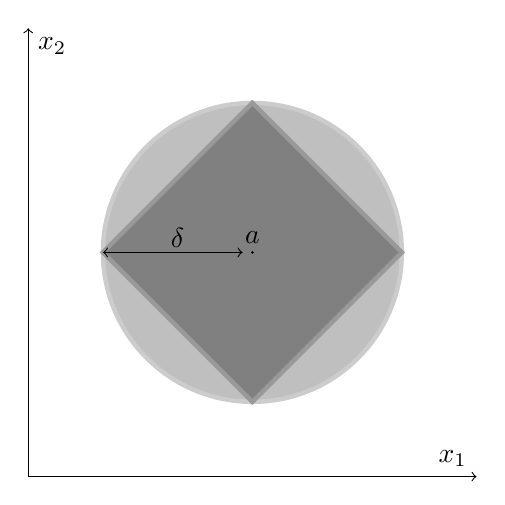
\begin{tikzpicture}
          \begin{axis}[ 
            ticks=none,
            axis lines = middle,
            axis line style={->},
            ymin=0, ymax=3,
            xmin=0, xmax=3,
            xlabel={$x_{1}$},
            ylabel={$x_{2}$},
            axis equal image,
            disabledatascaling
            ]
            \filldraw [ultra thick,fill=black!25!white, draw=black!20!white] (1.5,1.5) circle [radius=1];
            \filldraw[ultra thick,fill=black!50!white, draw=black!40!white] (0.5,1.5) -- (1.5,2.5) -- (2.5,1.5) -- (1.5,0.5) -- cycle;
            \fill [fill=black] (1.5,1.5) circle [radius=0.01];
            \draw (1.5,1.6) node {$a$};
            \draw (1.5,1.5) node {} edge[<->] (0.5,1.5);
            \draw (1,1.6) node {$\delta$};
          \end{axis}
        \end{tikzpicture}
        \caption{Een illustratie in $\mathbb{R}^{2}$}
      \end{figure}

    \item $\Leftarrow$\\
      Omgekeerd moeten we voor $r_{1}$ eenvoudigweg $\frac{r}{\sqrt{p}}$ nemen:
      \[ \forall x,y \in A:\ B_{1}(x,r) = \sum_{i=1}^{p}|x_{i}-y_{i}| \le \sqrt{\sum_{i=1}^{p}1} \sqrt{\sum_{i=1}^{p}|x_{i}-y_{i}|} = \sqrt{p}d(x,y) \]

      \begin{figure}[H]
        \centering
        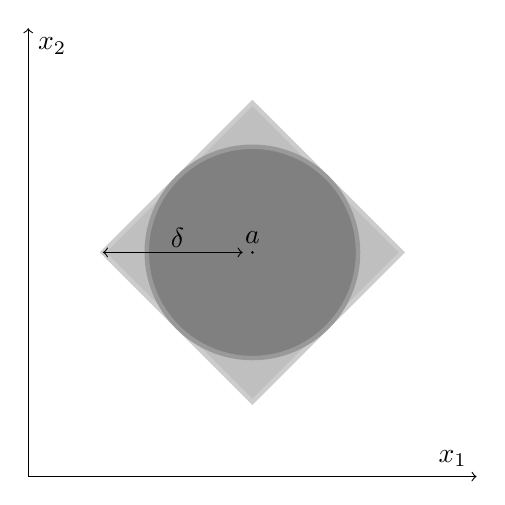
\begin{tikzpicture}
          \begin{axis}[ 
            ticks=none,
            axis lines = middle,
            axis line style={->},
            ymin=0, ymax=3,
            xmin=0, xmax=3,
            xlabel={$x_{1}$},
            ylabel={$x_{2}$},
            axis equal image,
            disabledatascaling
            ]
            \filldraw[ultra thick,fill=black!25!white, draw=black!20!white] (0.5,1.5) -- (1.5,2.5) -- (2.5,1.5) -- (1.5,0.5) -- cycle;
            \filldraw [ultra thick,fill=black!50!white, draw=black!40!white] (1.5,1.5) circle [radius=1/sqrt(2)];
            \fill [fill=black] (1.5,1.5) circle [radius=0.01];
            \draw (1.5,1.6) node {$a$};
            \draw (1.5,1.5) node {} edge[<->] (0.5,1.5);
            \draw (1,1.6) node {$\delta$};
          \end{axis}
        \end{tikzpicture}
        \caption{Een illustratie in $\mathbb{R}^{2}$}
      \end{figure}
    \end{itemize}
  \end{proof}
\end{st}

\subsubsection{De $d_\infty$- of maximummetriek op $\mathbb{R}^p$}
\label{sec:de-d_infty-maxim}

\begin{vb}
  $\mathbb{R}^{p}$, uitgerust met de volgende functie als metriek, is een metrische ruimte:
  \[ d_{\infty}:\ \mathbb{R}^{p}\times\mathbb{R}^{p}\rightarrow (x,y) \mapsto d_{\infty}(x,y)=\max_{i}|x_{i}-y_{i}| \]
  We noemen dit de \term{maximummetriek}.
\extra{bewijs}
  \begin{figure}[H]
    \centering
    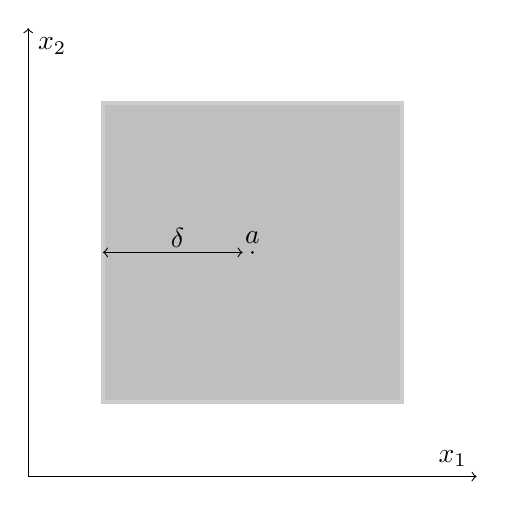
\begin{tikzpicture}
      \begin{axis}[ 
        ticks=none,
        axis lines = middle,
        axis line style={->},
        ymin=0, ymax=3,
        xmin=0, xmax=3,
        xlabel={$x_{1}$},
        ylabel={$x_{2}$},
        axis equal image,
        disabledatascaling
        ]
        \filldraw[ultra thick,fill=black!25!white, draw=black!20!white] (0.5,2.5) -- (2.5,2.5) -- (2.5,0.5) -- (0.5,0.5) -- cycle;
        \fill [fill=black] (1.5,1.5) circle [radius=0.01];
        \draw (1.5,1.6) node {$a$};
        \draw (1.5,1.5) node {} edge[<->] (0.5,1.5);
        \draw (1,1.6) node {$\delta$};
      \end{axis}
    \end{tikzpicture}
    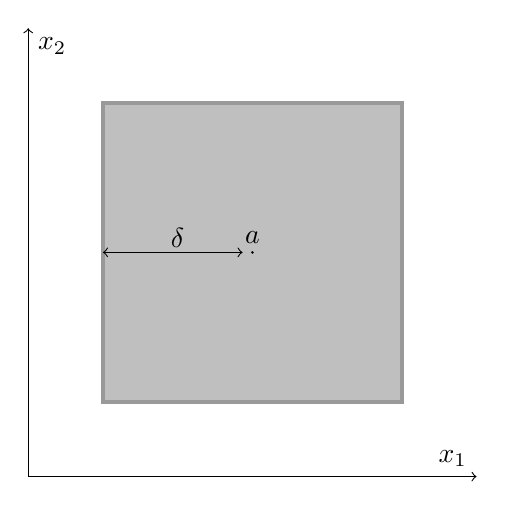
\begin{tikzpicture}
      \begin{axis}[ 
        ticks=none,
        axis lines = middle,
        axis line style={->},
        ymin=0, ymax=3,
        xmin=0, xmax=3,
        xlabel={$x_{1}$},
        ylabel={$x_{2}$},
        axis equal image,
        disabledatascaling
        ]
        \filldraw[ultra thick,fill=black!25!white, draw=black!40!white] (0.5,2.5) -- (2.5,2.5) -- (2.5,0.5) -- (0.5,0.5) -- cycle;
        \fill [fill=black] (1.5,1.5) circle [radius=0.01];
        \draw (1.5,1.6) node {$a$};
        \draw (1.5,1.5) node {} edge[<->] (0.5,1.5);
        \draw (1,1.6) node {$\delta$};
      \end{axis}
    \end{tikzpicture}
    \caption{Een open bol en een gesloten bol in $\mathbb{R}^{2},d_{\infty}$}
  \end{figure}
\end{vb}

\begin{st}
  Elke deelverzameling $A\subseteq \mathbb{R}^{p}$ is open voor de gewone metriek als en slechts als ze $d_{1}$-open is.

  \begin{proof}
    We moeten bewijzen dat er voor elke open bol $B(x,r)$ voor de gewone metriek een $d_{\infty}$-open bol $B_{\infty}(x,r_{1})$ bestaat met hetzelfde middelpunt die erin ligt en omgekeerd.
    \begin{itemize}
    \item $\Leftarrow$\\
      Kies $r_{\infty} = \frac{1}{\sqrt{p}}r$:
      \extra{bewijs}

      \begin{figure}[H]
        \centering
        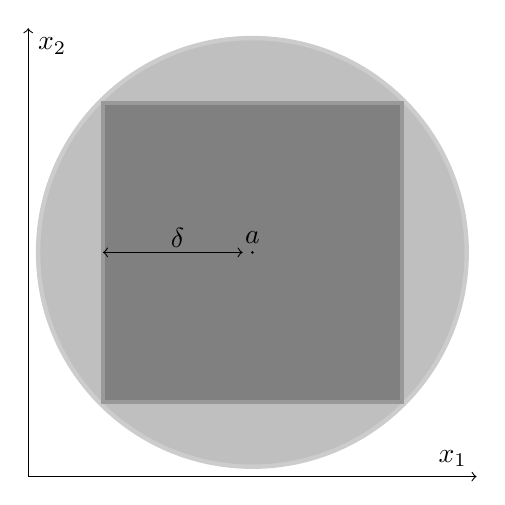
\begin{tikzpicture}
          \begin{axis}[ 
            ticks=none,
            axis lines = middle,
            axis line style={->},
            ymin=0, ymax=3,
            xmin=0, xmax=3,
            xlabel={$x_{1}$},
            ylabel={$x_{2}$},
            axis equal image,
            disabledatascaling
            ]
            \filldraw [ultra thick,fill=black!25!white, draw=black!20!white] (1.5,1.5) circle [radius=sqrt(2)+0.02];
            \filldraw[ultra thick,fill=black!50!white, draw=black!40!white] (0.5,2.5) -- (2.5,2.5) -- (2.5,0.5) -- (0.5,0.5) -- cycle;
            \fill [fill=black] (1.5,1.5) circle [radius=0.01];
            \draw (1.5,1.6) node {$a$};
            \draw (1.5,1.5) node {} edge[<->] (0.5,1.5);
            \draw (1,1.6) node {$\delta$};
          \end{axis}
        \end{tikzpicture}
        \caption{Een illustratie in $\mathbb{R}^{2}$}
      \end{figure}

    \item $\Rightarrow$\\
      Kies $r = r_{\infty}$:
      \extra{bewijs}

      \begin{figure}[H]
        \centering
        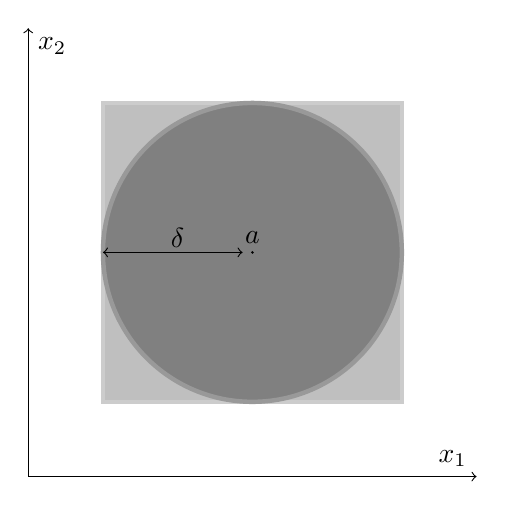
\begin{tikzpicture}
          \begin{axis}[ 
            ticks=none,
            axis lines = middle,
            axis line style={->},
            ymin=0, ymax=3,
            xmin=0, xmax=3,
            xlabel={$x_{1}$},
            ylabel={$x_{2}$},
            axis equal image,
            disabledatascaling
            ]
            \filldraw[ultra thick,fill=black!25!white, draw=black!20!white] (0.5,2.5) -- (2.5,2.5) -- (2.5,0.5) -- (0.5,0.5) -- cycle;
            \filldraw [ultra thick,fill=black!50!white, draw=black!40!white] (1.5,1.5) circle [radius=1];
            \fill [fill=black] (1.5,1.5) circle [radius=0.01];
            \draw (1.5,1.6) node {$a$};
            \draw (1.5,1.5) node {} edge[<->] (0.5,1.5);
            \draw (1,1.6) node {$\delta$};
          \end{axis}
        \end{tikzpicture}
        \caption{Een illustratie in $\mathbb{R}^{2}$}
      \end{figure}

    \end{itemize}
  \end{proof}
\end{st}

\subsubsection{De spoorwegmetriek op $\mathbb{R}^p$}
\label{sec:de-spoorw-op}

\begin{vb}
  $\mathbb{R}^{p}$, uitgerust met de volgende functie als metriek, is een metrische ruimte:
  \[
  d_{NMBS}:\ \mathbb{R}^{p}\times\mathbb{R}^{p}\rightarrow (x,y) \mapsto d_{NMBS}(x,y)=
  \begin{cases}
    \|x-y\| &\text{ als $x$ en $y$ lineair afhankelijk zijn}\\
    \|x\|+\|y\| &\text{ als $x$ en $y$ lineair onafhankelijk zijn}
  \end{cases}
  \]
  We noemen dit de \term{spoorwegmetriek}.
\extra{bewijs}
  \begin{figure}[H]
    \centering
    \begin{tikzpicture}
      \begin{axis}[ 
        ticks=none,
        axis lines = middle,
        axis line style={->},
        ymin=-1.5, ymax=2.5,
        xmin=-1.5, xmax=2.5,
        xlabel={$x_{1}$},
        ylabel={$x_{2}$},
        axis equal image,
        disabledatascaling
        ]
        \filldraw [ultra thick,fill=black!25!white, draw=black!20!white] (0,0) circle [radius=1];
        \fill [fill=black] (1.1,0.2) circle [radius=0.01];
        \draw [(-),color=black] (2.2,0.4) -- (0,0);
        \draw (1.1,0.4) node {$a$};
      \end{axis}
    \end{tikzpicture}
    \begin{tikzpicture}
      \begin{axis}[ 
        ticks=none,
        axis lines = middle,
        axis line style={->},
        ymin=0, ymax=2.5,
        xmin=0, xmax=2.5,
        xlabel={$x_{1}$},
        ylabel={$x_{2}$},
        axis equal image,
        disabledatascaling
        ]
        \fill [fill=black] (1.0,0.5) circle [radius=0.01];
        \draw [(-),color=black] (0.5,0.25) -- (1.5,0.75);
        \draw (1.1,0.4) node {$a$};
      \end{axis}
    \end{tikzpicture}
    \caption{Twee open bollen in $\mathbb{R}^{2},d_{NMBS}$ van verschillende straal}
  \end{figure}
\end{vb}

\subsection{Metrieken op rijruimten}
\label{sec:metr-op-rijr}

\begin{de}
  We noteren met $\mathbb{R}^{\mathbb{N}}$ de verzamelingen van alle rijen in $\mathbb{R}$.
  Merk op dat $\mathbb{R}^{\mathbb{N}}$ een vectorruimte is over $\mathbb{R}$.
\end{de}

\begin{vb}
  $\mathbb{R}^{\mathbb{N}}$, uitgerust met de volgende functie als metriek, is een metrische ruimte:
  \[ d:\ \mathbb{R}^{\mathbb{N}} \times \mathbb{R}^{\mathbb{N}} \rightarrow \mathbb{R}^{+}:\ ((x_{n})_{n},(y_{n})_{n}) \mapsto \sum_{n=0}^{+\infty}\frac{|x_{n}-y_{n}|}{2^{n}(1+|x_{n}-y_{n}|)} \]
\extra{bewijs en bewijs waarom dit goed gedefinieerd is}
\end{vb}

\begin{vb}
  Noteer met $l^{\infty}(\mathbb{N})$ het volgende:
  \[ l^{\infty}(\mathbb{N}) = \{ (x_{n})_{n} \in \mathbb{R}^{\mathbb{N}} \mid (x_{n})_{n} \text{ is begrensd.}\} \]
  $l^{\infty}$, uitgerust met de volgende functie als metriek, is een metrische ruimte:
  \[ d:\ \mathbb{R}^{\mathbb{N}} \times \mathbb{R}^{\mathbb{N}} \rightarrow \mathbb{R}^{+}:\ ((x_{n})_{n},(y_{n})_{n}) \mapsto \sup\{|x_{n}-y_{n}| \mid n\in \mathbb{N}\} \]
\extra{bewijs}
\end{vb}

\subsection{Metrieken op functieruimten}
\label{sec:metr-op-funct}

\begin{de}
  Zij $X$ een gesloten, begrensd deel van $\mathbb{R}^{p}$. Dan noteren we met $C(X)$ de vectorruimte van de continue functies van $X$ naar $\mathbb{R}$.
\end{de}

\begin{de}
  Zij $\interval{a}{b}$ een gesloten, begrensd interval in $\mathbb{R}$, dan noteren we met $C(\interval{a}{b})$ de vectorruimte van de continue functies van $\interval{a}{b}$ naar $\mathbb{R}$.
\end{de}

\begin{vb}
  Zij $X$ een gesloten en begrensde deelverzameling van $\mathbb{R}^{p}$, dan is $C(X)$, uitgerust met de volgende functie als metriek, een metrische ruimte:
  \[ d_{\infty}:\ C(x)\times C(X)\rightarrow \mathbb{R}^{+}:\ (f,g) \mapsto d_{\infty}(f,g) = \sup \{ |f(x)-g(x)| \mid x \in X \} \]

  \extra{bewijs}
\end{vb}

\begin{opm}
  Merk op dat dit goed gedefinieerd is omdat $|f(x)-g(x)|$ voor continue functies op een gesloten, begrensd deel steeds begrensd blijft. \needed
\end{opm}

\begin{vb}
  Een open bol $B(f,\delta)$ in $C(\interval{a}{b})$ ziet er als volgt uit:
  \[ B(f,\delta) = \{ g \in C(\interval{a}{b} \mid  \forall x\in \interval{a}{b}:\ |g(x)-f(x)|< \delta \]
  \begin{figure}[H]
    \centering
    \begin{tikzpicture}[scale=.75]
      \begin{axis}[ymin=-0.5, ymax=4, xmin=-2.9, xmax=2.9, no markers]
        \addplot[smooth,color=red,thick,domain=-3:-1]{-x};
        \addplot[smooth,color=red,thick,domain=-1:1]{x^2};
        \addplot[smooth,color=red,thick,domain=1:3]{x^3};
        \addplot[name path=A,smooth,color=black!20,thick,domain=-3:-1]{-x+0.25};
        \addplot[name path=B,smooth,color=black!20,thick,domain=-3:-1]{-x-0.25};
        \addplot[black!20] fill between[of=A and B];
        \addplot[name path=A,smooth,color=black!20,thick,domain=-1:1]{x^2+0.25};
        \addplot[name path=B,smooth,color=black!20,thick,domain=-1:1]{x^2-0.25};
        \addplot[black!20] fill between[of=A and B];
        \addplot[name path=A,smooth,color=black!20,thick,domain=1:3]{x^3+0.25};
        \addplot[name path=B,smooth,color=black!20,thick,domain=1:3]{x^3-0.25};
        \addplot[black!20] fill between[of=A and B];
      \end{axis}
    \end{tikzpicture}
    \caption{ Een illustratie van een open bol in $C(\interval{3}{3})$ rond een functie voor $p=1$. }
  \end{figure}

  \noindent
  Merk op dat dit slechts een illustratie is.
  Elke functie die volledig binnen de $\delta$-strook ligt, ligt binnen de open bol.
  Merk ook op dat de strook overal even breed is, ookal lijkt ze smaller voor een sterker stijgend deel van de functie.
\end{vb}

\begin{vb}
  Zij $f_{1},f_{2}:\ \interval{0}{1} \rightarrow \mathbb{R}$ twee continue functies met de volgende eigenschap
  \[ \forall t\in \interval{0}{1}:\ f_{1}(t) < f_{2}(t) \]
  Benoem een deelverzameling $A$ van $C(\interval{0}{1})$ als volgt:
  \[ A = \{ f\in C(\interval{0}{1}) \mid \forall t\in \interval{0}{1}:\ f_{1}(t) < f(t) < f_{2}(t) \} \]
  $A$ is dan $d_{\infty}$ open.

  \begin{proof}
    Kies een willekeurige $f\in A$.
    Voor alle $t\in \interval{0}{1}$ is $f(t) - f_{1}(t)$ strikt positief.
    Omdat $f-f_{1}$ continu is\prref{pr:optelling-continu} en $\interval{0}{1}$ gesloten\stref{st:gesloten-interval-gesloten} en begrensd, bestaat er een $r_{1}\in\mathbb{R}_{0}^{+}$ zodat $\forall t\in \interval{0}{1}:\ f(t)-f_{1}(t) > r_{1}$ geldt.
    Analoog bestaat er een $r_{2}\in \mathbb{R}^{+}$ zodat $\forall t\in \interval{0}{1}:\ f_{2}(t) -f(t) > r_{2}$
    Noem nu $r=\min\{r_{1},r_{2}\}$ en kies een willekeurige $g\in B_{\infty}(f,r)$, dan geldt het volgende en zit $g$ dus in $A$.
    \[ \forall t\in \interval{0}{1}:\ f_{1}(t) < f(t) - r_{1} \le f(t) - r < g(t) < f(t) + r \le f(t) + r_{2} < f_{2}(t) \]

    \begin{figure}[H]
      \centering
      \begin{tikzpicture}
        \begin{axis}[ymin=-1.1, ymax=1.1, xmin=-0.1, xmax=1.1, no markers]
          \addplot[name path=A,smooth,color=red,ultra thick,domain=0:1]{sin(150*x+60)};
          \addplot[name path=B,smooth,color=red,ultra thick,domain=0:1]{cos(150*x+60)};
          \addplot[black!20] fill between[of=A and B];

          \addplot[smooth,domain=0:1]{-1.45*x^2+0.75};
          \addplot[name path=C,smooth,color=black!30,thick,domain=0:1]{-1.5*x^2+0.75+0.1};
          \addplot[name path=D,smooth,color=black!30,thick,domain=0:1]{-1.5*x^2+0.75-0.1};
          \addplot[black!40] fill between[of=C and D];
        \end{axis}
      \end{tikzpicture}
      \caption{ Een illustratie van de situatie voor twee gekozen functies (rood), een willekeurige functie in $A$ (zwart) en een strook er rond om een open bol voor te stellen.}
    \end{figure}
  \end{proof}
\end{vb}


\begin{st}
  Een rij $(f_{n})_{n}$ in $C(X)$ zal volgens de $d_{\infty}$ metriek convergeren naar een $f\in C(X)$ als en slechts als $(f_{n})_{n}$ uniforum naar $f$ convergeert.

\extra{bewijs: ookal is het al duidelijk}
Hint uit les: zie forum, Eline heeft dit uitgeschreven.
Let wel op de ongelijheid met het supremum.
\end{st}

\begin{vb}
  Beschouw de rij functies $(f_{n})_{n}$ in $C(\interval{0}{1})$ gegeven als volgt:

  \noindent
  \begin{minipage}{.45\textwidth}
    \begin{figure}[H]
      \centering
      \begin{tikzpicture}[scale=.75]
        \begin{axis}[ymin=-1.1, ymax=1.1, xmin=-0.1, xmax=1.1]
          \foreach \i in {1,...,10}
          {
            \addplot[smooth,domain=0:(1/(2*\i))]{2*\i*x};
            \addplot[smooth,domain=(1/(2*\i)):(1/\i)]{2-2*\i*x};
            \addplot[smooth,domain=(1/(\i)):1.1]{0};
          }
          \addplot[smooth,color=red,ultra thick,domain=-3:3]{0};
          \addplot[soldot,color=red] coordinates {(0,0)};
        \end{axis}
      \end{tikzpicture}
    \end{figure}
  \end{minipage}
  \begin{minipage}{.45\textwidth}
  \[
  f_{n}: \mathbb{R} \rightarrow \mathbb{R}:\ x \mapsto
  \left\{
    \begin{array}{rl}
      2nx   & \text{ als } x \in \interval[open right]{0}{\frac{1}{2n}}\\
      2-2nx & \text{ als } x \in \interval{\frac{1}{2n}}{\frac{1}{n}}\\
      0     & \text{ als } x \in \interval[open left ]{\frac{1}{n}}{1}\\
    \end{array}
  \right.
  \]
  \[ f: \mathbb{R} \rightarrow \mathbb{R}:\ x \mapsto 0 \]
  \end{minipage}
  
  Deze rij convergeert niet voor de $d_{\infty}$-metriek want ze convergeert niet uniform.
  Volgens de $d_{1}$-metriek convergeert deze rij echer wel naar de nulfunctie.
\end{vb}

\begin{vb}
  Beschouw de functie $I$ als volgt:
  \[ I:\ C(\interval{a}{b}) \rightarrow \mathbb{R}:\ f \mapsto \int_{a}^{b}f(x)\ dx \]
  $I$ is continu als we op $C(\interval{a}{b})$ de $d_{\infty}$-metriek beschouwen en op $\mathbb{R}$ de gewone metriek.
\extra{bewijs}
\end{vb}

\begin{vb}
  Zij $\interval{a}{b}$ een gesloten en begrensd interval, dan is $C(\interval{a}{b})$,, uitgerust met de volgende functie als metriek, een metrische ruimte:
  \[ d_{1}:\ C(\interval{a}{b})\times C(\interval{a}{b}) \rightarrow \mathbb{R}^{+}:\ (f,g) \mapsto \int_{a}^{b}|f(x)-g(x)|dx \]
\extra{bewijs}
\end{vb}

\begin{opm}
  In deze metrische ruimte is het moeilijk om open bollen te tekenen, het inwendige van een deel van $C(\interval{a}{b})$ is namelijk seeds leeg.
\end{opm}

\begin{vb}
  Zij $\interval{a}{b}$ een gesloten begrensd interval, dan is $C(\interval{a}{b})$, uitgerust met de volgende functie als metriek, een metrische ruimte:
  \[ d_{2}:\ C(\interval{a}{b})\times C(\interval{a}{b}) \rightarrow \mathbb{R}^{+}:\ (f,g) \mapsto \sqrt{\int_{a}^{b}|f(x)-g(x)|dx} \]
  \extra{bewijs}
  Hint uit de les: het bewijs reduceert zich tot dit:
  \[ \left|\int_{a}^{b}f(x)g(x)\right| < \left(\int_{a}^{b}f(x)^{2}\ dx \right) \left(\int_{a}^{b}g(x)^{2}\ dx \right) \]
  Los hiervoor volgende ongelijkheid uit de genormeerde vectorruimte op met een discriminant.
  \[ \left\| v+\lambda w \right\| > 0 \]
\end{vb}

\begin{vb}
  De verzameling $A$ als volgt is een voorbeeld van een deel van $C(\interval{0}{1})$ dat begrensd is voor $d_{1}$, maar niet voor $d_{\infty}$.
  \[ A = \{ f \in C(\interval{0}{1}) \mid \int_{0}^{1}f(x)dx = 1 \]

  \begin{proof}
    De $d_{1}$ afstand is begrensd door $1$, maar de $d_{2}$ afstand is onbegrensd.
  \end{proof}
\end{vb}

\begin{st}
  $\forall f,g \in C(\interval{a}{b}):\ d_{1}(f,g) \le d_{\infty}(f,g)$
\extra{bewijs}
\end{st}

\begin{de}
  Noem de verzameling functies $f:\ \mathbb{R} \rightarrow \mathbb{R}$ die in beide oneindigheden naar $0$ gaan: $C_{0}(\mathbb{R})$.
\end{de}

\begin{vb}
  De functie $d$ als volgt, is niet alleen geen metriek voor $C_{0}(\mathbb{R})$, ze is ook niet goed gedefinieerd.
  \[ \int_{-\infty}^{+\infty}|f(x)-g(x)|\ dx \]
  De integraal bestaat immers niet steeds.
\end{vb}

\begin{vb}
  De functie $d$ als volgt, is een metriek voor $C_{0}(\mathbb{R})$.
  \[ d(f,g) = \int_{-\infty}^{+\infty}\frac{|f(x)-g(x)|}{1+x^{2}}\ dx \]
 \extra{bewijs}
\end{vb}


\subsection{Het product van metrische ruimten}
\label{sec:het-product-van}

\extra{product van metrische ruimten}

\subsection{Genormeerde vectorruimten}
\label{sec:genorm-vect}

\begin{de}
  Zij $(\mathbb{R},V,+)$ een vectorruimte, dan is een \term{norm} op $V$ een afbeelding als volgt:
  \[ \|\cdot\|:\ V \rightarrow \mathbb{R}^{+}:\ v \mapsto \|v\| \]
  \begin{enumerate}
  \item $\forall v\in V:\ \|v\| = 0 \Leftrightarrow v=0$
  \item $\forall v\in V, \forall \lambda \in \mathbb{R}:\ \|\lambda v\| = |\lambda|\|v\|$
  \item $\forall v,w\in V:\ \|v+w\| < \|v\| + \|w\|$
  \end{enumerate}
\end{de}

\begin{de}
  Een vectorruimte $\mathbb{R},V,+$, uitgerust met een norm noemen we een \term{genormeerde vectorruimte}.
\end{de}

\begin{st}
  Een genormeerde vectorruimte $\mathbb{R},V,+,\|\cdot\|$, uitgerust met de volgende functie als metriek, vormt een metrische ruimte:
  \[ d:\ V \times V \rightarrow \mathbb{R}^{+}:\ (x,y) \mapsto \|x-y\| \]
\extra{bewijs}
\end{st}

\begin{st}
  Equivalente definitie voor begrensde delen in een genormeerde vectorruimte:
  Een deel $A$ van een genormeerde vectorruimte $\mathbb{R},V,+$ is begrensd als en slechts als er een $M \in \mathbb{R}^{+}$ bestaat als volgt:
  \[ \forall x\in A:\ \|x\| \le M \]
\extra{bewijs}
\end{st}

\subsection{Hausdorffmetriek}
\label{sec:hausdorffmetriek}

\begin{de}
  Voor een niet-lege deelverzameling $A$ van $\mathbb{R}^{p}$ en een $r\in \mathbb{R}^{+}$ definie\"eren we de $r$-omhullende $[A]_{r}$ van $A$ als volgt:
  \[ [A]_{r} = \{r \in \mathbb{R}^{p} \mid \exists a \in A:\ d(x,a) \le r \} \]
  Hierin staat $d$ voor de gewone euclidische metriek.
\end{de}

\begin{de}
  Noteer met $\mathcal{F}$ de verzameling van niet-lege gesloten en begrensde deelverzamelingen van $\mathbb{R}^{p}$.
  \[ \mathcal{F} = \{ A \mid A \subseteq \mathbb{R}^{p}, A \text{ is gesloten en begrensd } \} \]
\end{de}

\begin{de}
  We defini\"eren de \term{Hausdorffafstand} $h(F,G)$ tussen twee deelverzamelingen $F,G \in \mathcal{F}$ als volgt:
  \[ h(F,G) = \inf\{ r\in \mathbb{R}^{+} \mid F \subseteq [G]_{r} \text{ en } G \subseteq [F]_{r} \} \]
\end{de}

\begin{blem}
  \label{lem:omhullenden-in-elkaar}
  Zij $A \subseteq \mathbb{R}^{p}$ en $r,s\in\mathbb{R}^{+}$ met $r\ge s \ge 0$.
  \[ [A]_{s} \subseteq [A]_{r} \]

  \begin{proof}
    Dit volgt meteen uit de definitie:
    Kies een $x\in [A]_{s}$, dan bestaat er een $a\in A$ zodat $d(x,a) \le s$ geldt.
    Omdat $r \ge s$ geldt, geldt ook $d(x,a) \le r$ en dus zit $x$ ook in $[A]_{r}$.
  \end{proof}
\end{blem}

\begin{blem}
  Zij $A \subseteq \mathbb{R}^{p}$ en $r,s\in\mathbb{R}^{+}$:
  \[ \left[ [A]_{r}\right]_{s} \subseteq [A]_{r+s} \]

  \begin{proof}
    Kies een $x\in \left[[A]_{r}\right]_{s}$, dan bestaat er een $b\in [A]_{r}$ als volgt:
    \[ d(x,b) \le s \]
    Omdat $b$ in $[A]_{r}$ zit, bestaat er ook een $c\in A$ als volgt:
    \[ d(b,c) \le r \]
    We gebruiken nu de driehoeksongelijkheid:
    \[ d(x,c) \le d(x,b) + d(b,c) \le r + s \]
    $x$ behoort dus tot $[A]_{r+s}$.
  \end{proof}
\end{blem}

\begin{blem}
  Zij $F,G \in \mathcal{F}$ en $r=h(F,G)$.
  \[ F \subseteq [G]_{r} \text{ en } G \subseteq [F]_{r} \]

  \begin{proof}
    Kies een willekeurige $x\in F$.
    Omdat $r = h(F,G)$ geldt, zal volgens de definitie van $h$ het volgende gelden:\lemref{lem:omhullenden-in-elkaar}
    \[ F \subseteq [G]_{r+\frac{1}{n}}\]
    Er bestaat dus een rij punten $(y_{n})_{n}$ in $G$ met de volgende eigenschap:
    \[ \forall n \in \mathbb{N}:\ d(x,y_{n}) \le r + \frac{1}{n} \]
    Omdat $G$ gesloten en begrensd is, bestaat er een deelriij $(y_{n_{k}})_{k}$ die convergeert naar een $y\in G$.\stref{st:in-rp-gesloten-en-begrensd-itv-rijen}
    Voor deze $y$ zal $d(x,y) \le r$ gelden.
    We vinden dus dat $x$ in $[G]_{r}$ zit.
    $F$ moet dus een deel zijn van $[G]_{r}$ en omgekeerd is de redenering hetzelfde met de namen $F$ en $G$ omgewisseld.
  \end{proof}
\end{blem}

\begin{pr}
  De Hausdorffafstand $h$ is een metriek die $\mathcal{F},h$ een metrische ruimte maakt.

  \begin{proof}
    We gaan de eigenschappen van een metrische ruimte na.
    \begin{itemize}
    \item $\forall F,G\in \mathcal{F}:\ h(F,G) \ge 0$: Dit volgt meteen uit de definitie.
    \item $\forall F,G\in \mathcal{F}:\ h(F,G) = 0 \Leftrightarrow F = G$: Idem
    \item $h$ is symmetrisch: Dit zit vervat in de definitie.
    \item $h$ voldoet aan de driehoeksongelijkheid.
      Kies 3 elementen $F$, $G$ en $H$ uit $\mathcal{F}$.
      Noem $s=h(F,G)$ en $t=(G,H)$.
      Meteen vinden we het volgende:
      \[ G \subseteq [H]_{t} \quad\text{ en }\quad F \subseteq [G]_{s} \subseteq \left[[H_{t}]\right]_{s} \subseteq [H_{t+s}] \]
      Analoog vinden we $H \subseteq [F]_{t+s}$ en bijgevolg $h(F,H) \le s+t$.\needed
    \end{itemize}
  \end{proof}
\end{pr}

\begin{opm}
  Het is belangrijk dat de deelverzamelingen waartussen we de afstand meten gesloten en begrensd zijn.
  Stel immers dat \'e\'en ervan niet begrensd zou zijn, dan bestaat de Hausdorffafstand niet.
  Een $r$-omhulling heeft immers een eindige $r$ nodig om zinvel te zijn.
  Stel anderzijds dat de verzamelingen niet gesloten zouden zijn, dan bestaat het supremem in de definitie niet noodzakelijk.
\end{opm}

\begin{st}
  \[ \forall x,y \in \mathbb{R}^{p}:\ h(\{x\},\{y\}) = d(x,y) \]

  \begin{proof}
    
  \end{proof}
\end{st}
\begin{opm}
  We kunnen $\mathbb{R}^{p},d$ dus als deelruimte van $\mathcal{F},h$ via de inbedding $\mathfrak{i}$ als volgt:
  \[ \mathfrak{i}:\ \mathbb{R}^{p} \rightarrow \mathcal{F}:\ x \mapsto \{x\} \]
\end{opm}

\begin{vb}
  Beschouw $F_{1} = B\interval{x_{1}}{r_{1}}$ en $F_{2}= B\interval{x_{2}}{r_{2}}$.

\extra{bewijs: $h(F_{1},F_{2}) = d(x_{1},x_{2}) + |r_{1}-r_{2}|$.}
\end{vb}

\extra{voorbeelden van HDafstandberekeningen}

\begin{st}
  Een rij gesloten bollen $(B_{n})_{n}$ in $\mathbb{R}^{p}$ met middelpunten $x_{n}$ en stralen $r_{n}$ zal voor de Hausdorffmetriek convergeren naar een gesloten bol $B$ met middelpunt $x$ en straal $r$ als en slechts als $\lim_{n\rightarrow +\infty}x_{n}=x$ en $\lim_{n\rightarrow +\infty}r_{n} = r$ gelden.
\extra{bewijs}
Hint:
\begin{proof}
  \begin{lem}
    $\forall r,s \in \mathbb{R}^{+}:\ \left[B\interval{x}{r}\right]_{s} = B\interval{x}{r+s}$
  \end{lem}

  \begin{lem}
    $\forall r\in \mathbb{R}^{+}:\ B\interval{x}{r} \subseteq B\interval{y}{r+\|x-y\|}$
  \end{lem}
  Gevalsonderscheid.
\end{proof}
\end{st}

\begin{st}
  $(n)_{n}$ in $\mathbb{R}$ is voor de gewone metriek geen Cauchyrij maar wel voor de $d_{2}$-metriek.
\extra{bewijs}
\extra{wat met de $d_1$-metriek?}
\end{st}




\end{document}

%%% Local Variables:
%%% mode: latex
%%% TeX-master: t
%%% End:
